\chapter{Efficiency calculations}
\label{sec:Efficiency}

The reconstruction steps described in the Sec.~\ref{sec:Reconstruction} are not absolutely effective. The algorithms occasionally misinterpret particles and thus introduce the errors in the results. This margin of error is called the efficiency, and it is present for reconstructing both collision and MC data. But to be able to compare collision data to theoretical predictions, the efficiency in both cases should be the same, which is not the case. To remedy this, the so-called "efficiency correction factors" were introduces for every step of the reconstruction chain: for trigger efficiency ($\varepsilon_{TG}$), reconstruction efficiency ($\varepsilon_{Reco}$), identification efficiency ($\varepsilon_{ID}$), and isolation efficiency ($\varepsilon_{ISO}$). The correction factor for every efficiency is defined as a ratio $\varepsilon^{data}/\varepsilon^{MC}$.

All efficiencies are measured using the tag-and-probe method, which require two electrons, one of which should pass the tight identification and would be called "tag", and the other should pass the weak identification and would be called "probe". If the "probe" also passes the tight identification, it is called "passing probe", and it is called "failing probe". The efficiency is then calculated as a ratio of the passing probes to the whole amount of tags, and is usually calculated in 2D binning of $|\eta|$ and $p_{T}$.

In the following sections all the efficiencies would be discussed separately.

\section{Trigger efficiency}

The efficiency of the electron triggers was done with the use of the \Zee\ data which gives a clear selection of electrons with wide range in both $p_{T}$ and $\eta$. For the central-forward analysis one uses a single-electron trigger, but since we need two electrons for the tag-and-probe method, the trigger efficiency was calculated using the central-central \Zee\ data. To get that data, the usual \Zee\ CC cut chain was applied, but with ID and ISO cuts being changed to that, required from the central electrons from the \Zee\ CF and \Wen\ analyses. After that every electron was consecutively used as a "tag" and as a "probe", with the "tag" always being required to be matched to the single-electron trigger, and the efficiency of a successful match of the "probe" to the same trigger being evaluated.

The scale factors were calculated in three different mass windows of $70 \le m_{ee} \le 110$~GeV, $80 \le m_{ee} \le 100$~GeV, and $85 \le m_{ee} \le 95$~GeV, to vary the background level. The results from the middle mass window were used to define the central value of the scale factors, while the other two were used to derive a source of uncertainty. To evaluate the uncertainty further, a background subtraction via OS-SS pairs (opposite sign minus same sign) was performed. The central value was taken from the OS pairs and the full difference to the OS-SS sample was taken as another source of uncertainty.

The whole MC sample was divided in four periods corresponding to data periods B-H, I-J, K and L-M. Each of these MC periods is distinguishable by its unique LAr calorimeter and trigger setups, and should be used separately in order to calculate the scale factors which are valid only for that particular period. After propagation to the final cross section measurement using the combined ToyMC method (see sec.~\ref{sec:ZeeD_toymc}), the resulting uncertainty is typically $0.1\%$ only.

The calculated trigger efficiencies for the default single-electron triggers used in the analysis are presented in Fig.~\ref{fig:eff_trig}.

\begin{figure}
\center{
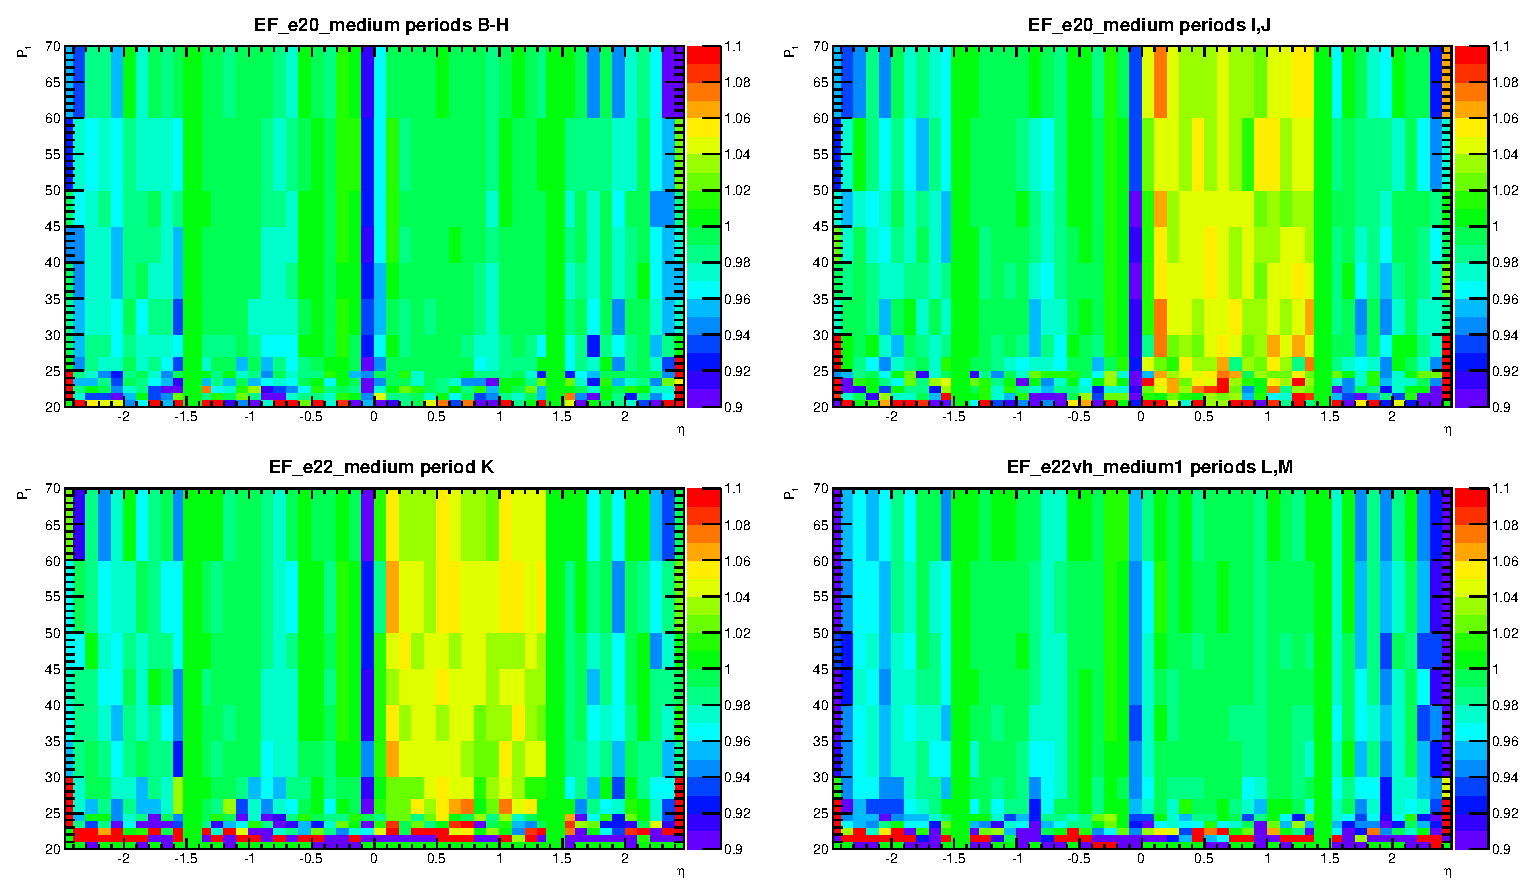
\includegraphics[width=1.0\textwidth]{figures/SingElTrigSFs2D.eps}
\caption{Scale factors for the default single-electron triggers used in the 2011 data.}
\label{fig:eff_trig}}
\end{figure}

\section{Reconstruction and identification efficiency}

There are three separate efficiencies that contribute to the electron identification, the efficiency of the cluster reconstruction algorithm, the efficiency of the electron reconstruction algorithm, and the efficiency of the electron identification algorithm. Every subsequent algorithm only works if its predecessors succeeded, so all the three efficiencies are tied together, and may be explored together.

\section{Isolation efficiency}
